%!TEX root = paper.tex

\section{System Architecture}

In this section we lay out the architecture of Flink as a software stack, and as a distributed system. While Flink's stack of APIs continues to grow, we can distinguish four main layers: deployment, core, APIs, and libraries.

\para{Flink's Runtime and APIS.} The core of Flink is the distributed dataflow engine, which executes dataflow programs. A Flink runtime program is a DAG of stateful operators connected with data streams. There are two core APIs in Flink: the DataSet API for processing finite data sets (often referred to as “batch processing”), and the DataStream API for processing potentially unbounded data streams (often referred to as “stream processing”). Flink’s core runtime engine can be seen as a streaming dataflow engine, and both the DataSet and DataStream APIs create runtime programs executable by the engine. As such, it serves as the common fabric to abstract both bounded (batch) and unbounded (stream) processing. On top of the core APIs, Flink bundles domain-specific libraries and APIs that generate DataSet and DataStream API programs (currently FlinkML, Gelly, and Table). 

A Flink cluster comprises of three types of processes: the client, the JobManager (JM - master), and one or more TaskManagers (RM - workers). The client takes the program code, transforms it to a runtime executable, and submits it to the JobManager. The compilation process involves a type extraction and checking phase that generates serializers and comparators for all used types. DataSet programs, also go through a cost-based query optimization phase, similar to the physical optimizations performed by relational query optimizers (more details in ???).

The JobManager is Flink’s master node. It coordinates all message-passing during job execution by sending heartbeats to the TaskManagers and receiving statistics, controls the tasks’ lifecycle, and coordinates checkpointing used for recovery. The actual data processing takes place in the TaskManagers that they execute several tasks in multiple threads, and maintain data structures shared by all tasks (e.g., buffer pools) executed by a TM. TMs communicate directly with each other using a multiplexed TCP connection per TM pair. 

\begin{figure}
\centering
	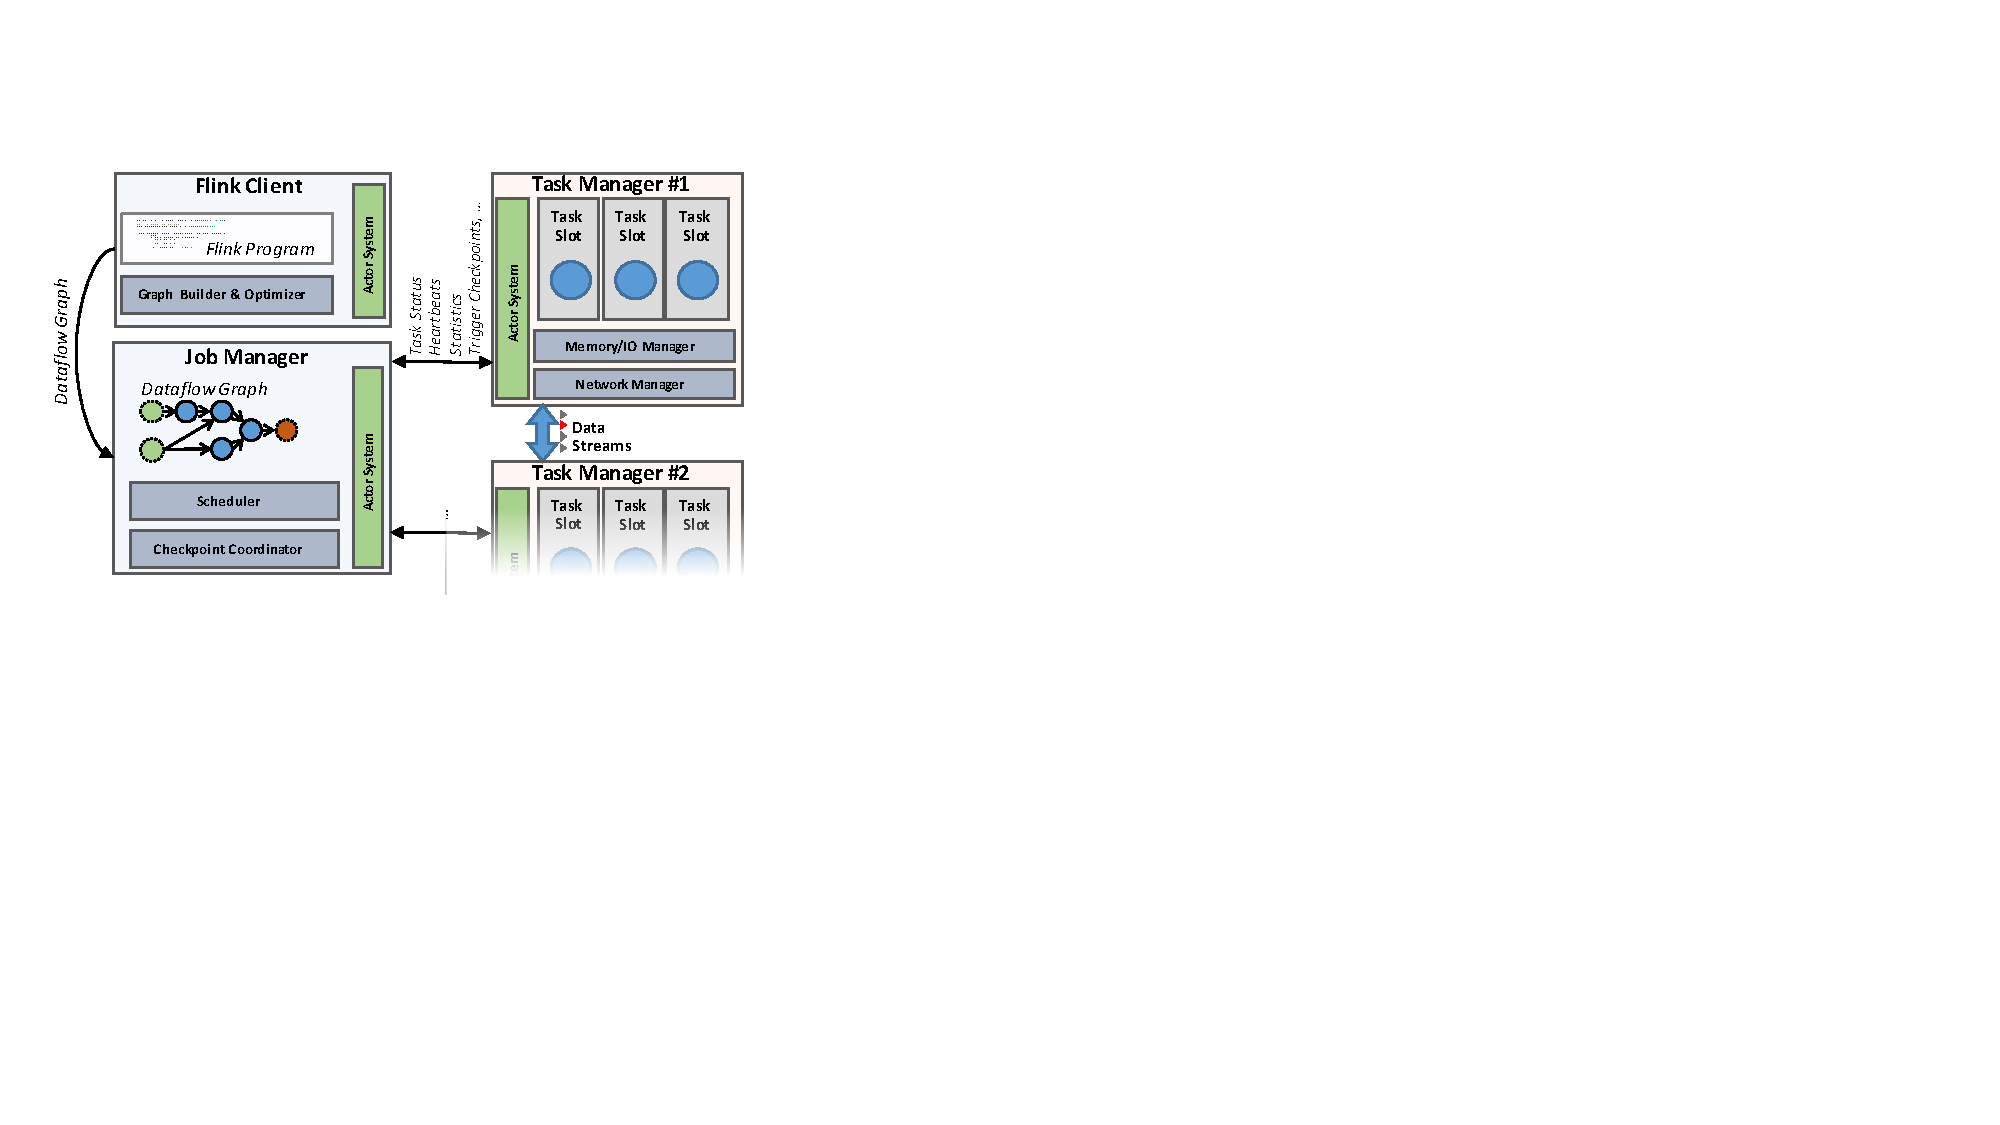
\includegraphics[width=.5\textwidth]{figs/architecture}
\caption{Flink's Process Model.}
\end{figure}

\begin{figure}[ht]
\centering     %%% not \center
\subfigure[The Flink software stack.]{\label{fig:FlinkStack}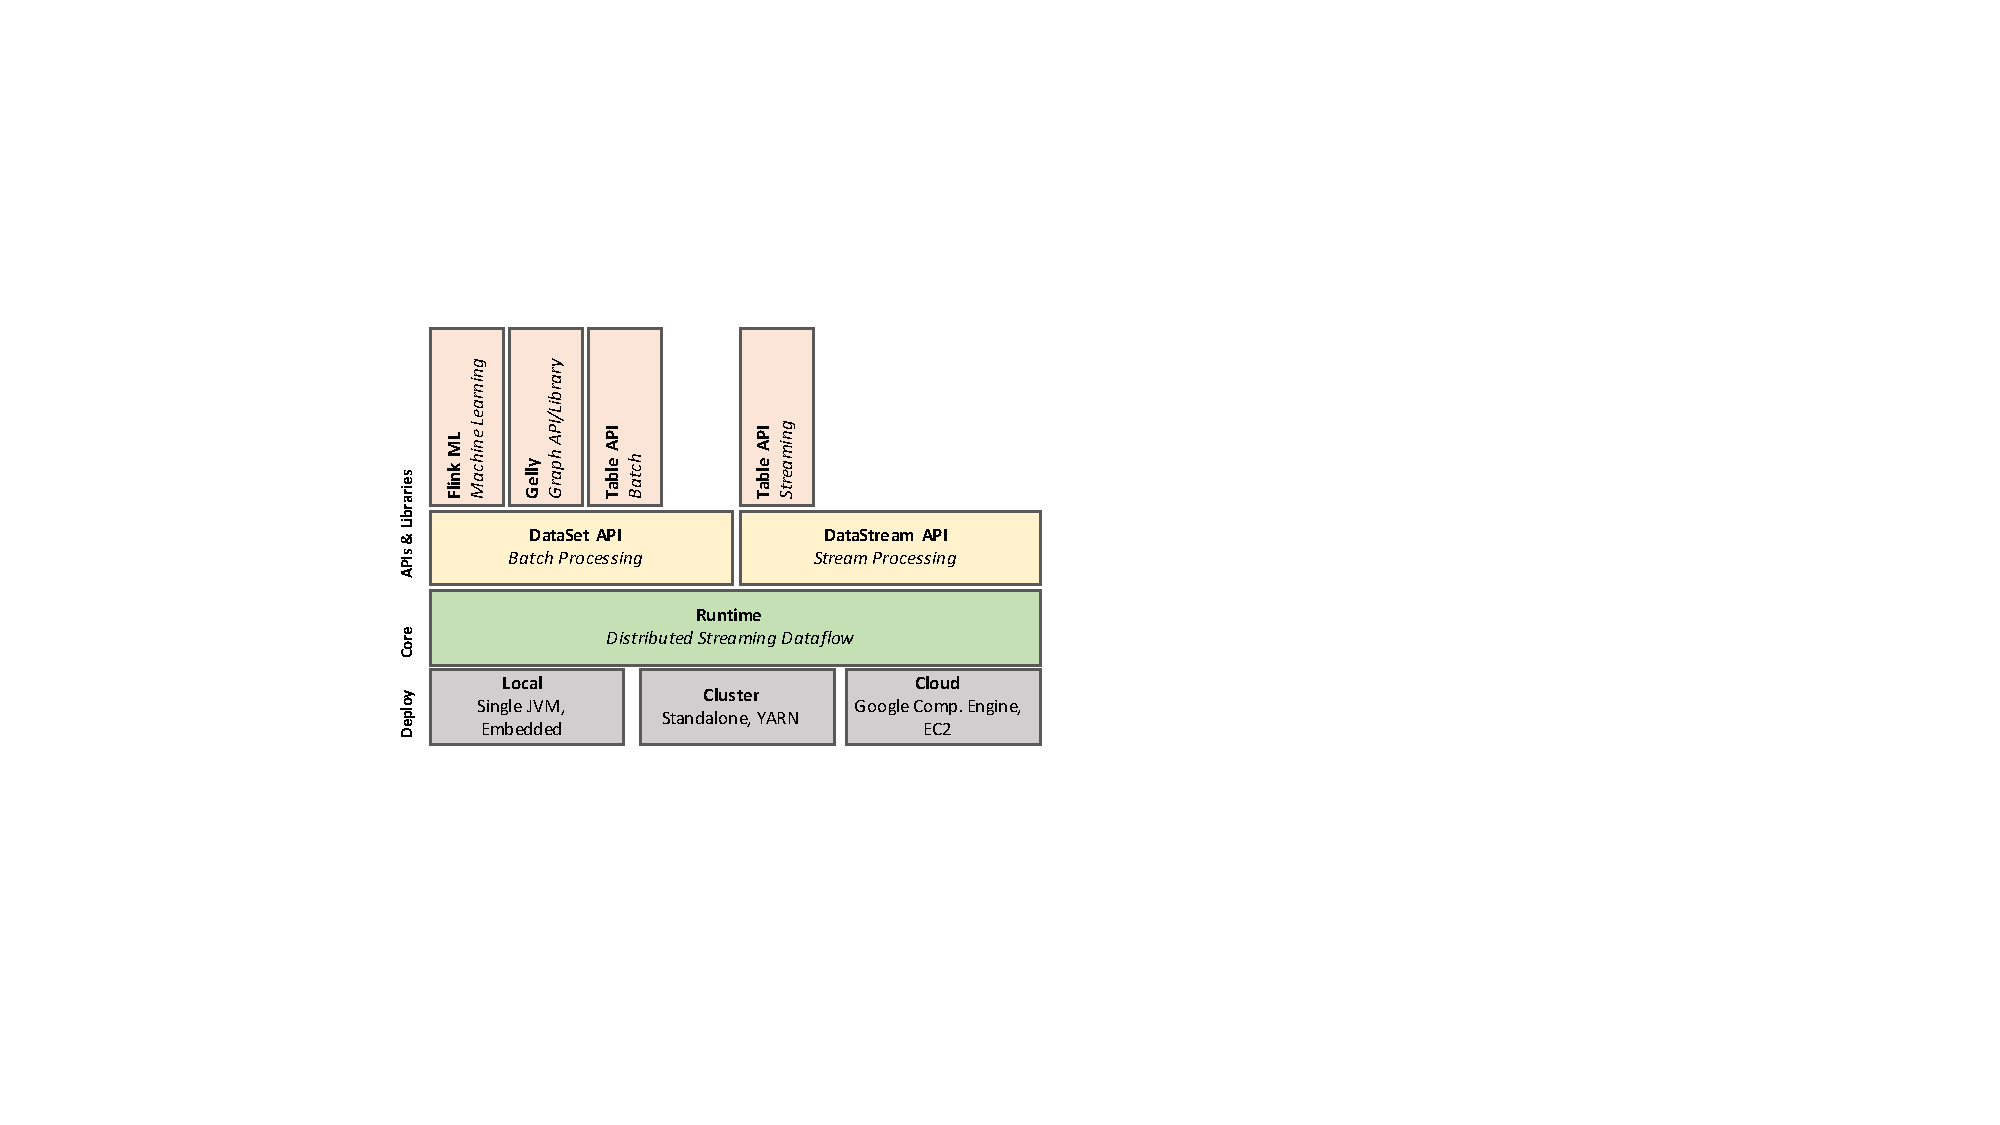
\includegraphics[width=.5\textwidth]{figs/stack.pdf}}
\subfigure[The JobGraph is the logical view of a Flink job.]{\label{fig:JobGraph}\begin{tikzpicture}
[shorten >=1pt,node distance=1.75cm,>=stealth',initial text=, font=\tiny]
\tikzstyle{op}=[circle, draw=blue!50,very thick,fill=blue!20, text width=0.5cm]
\tikzstyle{ir}=[cylinder, cylinder uses custom fill, cylinder body fill=orange!50, cylinder end fill=orange!50, shape border rotate=90, aspect=0.35, draw, minimum size=1cm, text width=0.5cm, align=center]

\node[op] (op_1) {~~~~~~~};
\node[ir] (ir_1) [right of = op_1] {~~~~~~~};
\node[op] (op_2) [right of = ir_1] {~~~~~~~};
\node[ir] (ir_2) [right of = op_2] {~~~~~~~};
\node[op] (op_3) [below of = op_2] {~~~~~~~};
\node[ir] (ir_3) [right of = op_3] {~~~~~~~};
\node[op] (op_4) [right of = ir_2] {~~~~~~~};
\node[op] (op_5) [right of = ir_3] {~~~~~~~};
			
\path[->] 	
			(op_1) 	edge node [above] {} (ir_1)
			(ir_1) 	edge node [above] {} (op_2)
			(op_2) 	edge node [above] {} (ir_2)
			(ir_2) 	edge node [above] {} (op_4)
			(op_3) 	edge node [above] {} (ir_3)
			(ir_3) 	edge node [above] {} (op_4)
			(ir_3) 	edge node [above] {} (op_5)
			;
\end{tikzpicture}}
\caption{Apache Flink architecture.}
\end{figure}
